\documentclass[11pt]{book}
\usepackage{geometry}        
\geometry{letterpaper}    
\usepackage[parfill]{parskip}  
\usepackage{graphicx}
\usepackage{caption}
\usepackage{subcaption}
\usepackage{amssymb}
\usepackage{epstopdf}
\usepackage{listings}
\usepackage{times}
\usepackage{float}
\usepackage{cleveref}

\usepackage[final]{pdfpages}


\DeclareGraphicsRule{.tif}{png}{.png}{`convert #1 `dirname #1`/`basename #1 .tif`.png}

\usepackage[colorlinks=true, pdfstartview=FitV, linkcolor=black, 
            citecolor=blue, urlcolor=blue]{hyperref}

\usepackage{tocloft}



\renewcommand\cftchapfont{\Large\bfseries}
\renewcommand\cftsecfont{\Large\bfseries}

%\renewcommand\cftchappagefont{\LARGE\bfseries}
%\renewcommand\cftsecpagefont{\LARGE}

\renewcommand\cftchapafterpnum{\par\addvspace{6pt}}
\renewcommand\cftsecafterpnum{\par\addvspace{6pt}}

% ------------------- Title and Author -----------------------------

\setlength\parindent{24pt}
\renewcommand{\baselinestretch}{1}
\linespread{1.5}

\begin{document}

\begin{titlepage}
    \begin{center}
                
        \Large
        \textbf{Intro Stat Shiny}
        
      
        \vspace{1cm}
       
        
        \Large
        Chelsey Legacy \\
        \vspace{0.25cm}
        Department of Statistics\\
          \vspace{0.25cm}
        Iowa State University\\
       
        
        \vspace{1cm}
               
           Creative Component\\
             \vspace{0.25cm}
           Spring 2017
           
           \vspace{2cm}
         
				\begin{center}
				\begin{tabular}{rl}
				Committee Members: & Amy G. Froelich, Major Professor\\
				 & W. Robert Stephenson \\
				 & Heike Hofmann\\
				\end{tabular}
				\end{center}
           
    \end{center}
\end{titlepage}







\begin{center}
\textbf{Abstract}
\end{center}
\newpage
\tableofcontents
\renewcommand\thechapter{\arabic{chapter}}
\renewcommand\thesection{\arabic{section}}
%\renewcommand\thesubsection{(\arabic{subsection})}

\newpage
\section{Introduction}
Over the past 30 years, technology has become an integral part of teaching undergraduate statistics courses. Statistical software packages like JMP, StatCrunch, R, and Minitab are used to teach students the skills to conduct data analysis. Some of these same programs plus Java web-based applets have been used to teach students concepts in introductory statistics, particularly sampling distributions and inferential topics. Instructors select technology platforms based on a number of concerns particular to their audience and institution. One recent option, R's Shiny applications, provides an easy to use and interactive interface for introductory statistics students. The application can run on any web browser, allowing students and instructors to use the app on mobile devices, tablets, Chromebooks, and computers, with no cost to the students or instructor. As a relatively new option for instructional technology, there are few resources available for the introductory statistics course using the Shiny application in R. In this paper, we will outline the creation of an R shiny app and supporting supplemental worksheets to be used in conjunction with the app for the introductory statistics course. The Shiny app includes resources for teaching concepts in inference for a population proportion, population mean, difference between two population proportions, and the difference between two population means; descriptive linear regression and correlation, and ANOVA.

In section 2, we will discuss the literature related to technology in the classroom, specifically as it relates to teaching concepts in introductory statistics. In section 3, the development of the Shiny app is detailed, and we discuss the supplemental worksheets in Section 4. Conclusions and details of future work appear in Section 5.
 
\section{Literature Review}
	   	
	Most undergraduate statistics courses make use of some sort of technology in the classroom from calculators to computer software programs.  All the available technology has the ability to simplify complex calculations in addition to making conceptual ideas more concrete.  These are two main features of technology that has helped make it a staple tool for statistics education.  Roy D. Pea provides an argument about why the computer as a cognitive technology is so important to the advancement in learning mathematics, in his article \emph{Cognitive Technologies for Mathematics Education} (1987).  Though his article focuses on the role of technology in math education there is a direct tie to statistics, in that he is discussing calculations and graphing data, both of which are essential elements of statistics courses.  He introduces cognitive technologies as ``any medium that helps transcend the limitations of the mind (e.g. attention to goals, short-term memory span), in thinking, learning, and problem-solving activities" (91). Computer applets and software are precisely the type of cognitive technologies being described that can help student thinking to go beyond just following formulas and returning answers.  
		
	  Pea goes on to describe this idea further,  ``a common feature to all these cognitive technologies is that they make external the intermediate products of thinking (e.g. output of the component steps in solving a complex algebraic equation), which can then be analyzed, reflected upon, and discussed" (Pea, 1987, p. 91).  With the help of computers, we are able to put thoughts and equations into visual and graphical representations that can then be viewed by many and discussed in an effort to clarify statistical concepts.  The main goal of this project was to be used in helping statistics students gain some insight and confidence in working with complex concepts.  Pea perfectly sums up this idea by saying that ``the dynamic and interactive media provided by computer software make gaining an intuitive understanding (traditionally the province of the professional mathematician) of the interrelationships among graphic, equational, and pictorial representations more accessible to the software user."(1987, p. 96)  Technologies such as R's Shiny web applications have the ability to provide insights to students through their interactivity and the output they provide that are not available through lectures or notes on a blackboard.
	 

The use of these technologies in the curriculum had a profound impact on the pedagogy of statistics. Chance et al. provide a discussion in  \emph{The Role of Technology in Improving Student Learning of Statistics} about how courses are changing format.  They specify that, "students are evaluated less on their ability to manipulate formulas and look up critical values, and more on their ability to select appropriate tools (e.g., choosing techniques based on the variables involved), assess the validity of different techniques, utilize graphical tools for exploration of data, deal with messier data sets, provide appropriate interpretations of computer output, and evaluate and communicate the legitimacy of their conclusions`` (p. 3).  They state, "technology has expanded the range of graphical and visualization techniques to provide powerful new ways to assist students in exploring and analyzing data and thinking about statistical ideas, allowing them to focus on interpretation of results and understanding concepts rather than computational mechanics`` (p. 3).    Though, technology has all the aforementioned benefits it is important that the technology should support the course learning objectives, and not restructure the objectives to pertain to learning the software.  Chance et al, argue that technology should not be used " merely for the sake of using technology",  but instead used for accessing, analyzing and interpreting large real data sets, automating calculations and processes, generating and modifying appropriate statistical graphics and models, performing simulations to illustrate abstract concepts and exploring 'what happens if...' type questions" (p.2-3).

There are increasingly many different software programs and applets available to supplement introductory statistics courses.  Chance et al describe how " the types of technology used in statistics and probability instruction can be broken into several categories: Statistical software packages, educational software, spreadsheets, applets/standalone applications, graphing calculators, multimedia materials, and data repositories." (p.4) These options all have advantages and drawbacks highlighted in the article by Chance et al.  


Choosing among these various options largely depends on the content of your course, your students expected competency on such programs, and funding available.  Fathom, Minitab, and JMP are all point and click programs that allow users to enter and manipulate data, and they will provide graphical and summary statistics of the data.  The drawback of such programs is that they cost the institution or the students money for downloads of the software.  Of course R and R studio can also provide the graphical output and summary statistics needed by the students and they are available for free.  However, with both R and the point and click software there is a learning curve for the students.    Many students may enter the course with little to no programming or even basic computer skills.   To avoid the course becoming inaccessible to those students, the software chosen should be fairly straightforward and require no previous knowledge.   Use of complex programs provides the problem of the students focusing so much on learning the software that they lose sight of the statistical concepts they are actually supposed to be learning.  

 In addition to software, there are many great web based java applets that are free to use and provide conceptual frameworks for simulations, p-values, and other intro stat concepts made available by Rossman and Chance (2004).  These are helpful additions to already created lecture slides and materials, however they do not provide any supplemental materials that can help guide student interaction with the applets.  As pointed out by Doi et al in \emph{Web Application Teaching Tools for Statistics Using R and Shiny}, there are a multitude of available software and programs, however eventually an instructor may have difficulty finding an applet or software that perfectly suits their needs for their lectures (p. 1).
 
 With monetary and time costs to consider, R`s Shiny app technology is a great option for technology to incorporate into the classroom.  R`s package allows the developer to create an interactive app that is point and click based, and allows the user to perform complex tasks with the click of a button.  In Doi et al's article the authors provide a discussion on the advantages of using Shiny in the classroom. One of the main advantages is that the user never has to engage in writing or seeing the code if the developer chooses.  The developer is the only one that must have a basic understanding of coding in R to get the app successfully running (p. 6, Doi et al, 2016).
 The authors explain that, "all adjustments in the app are done by moving sliders or clicking buttons and corresponding updates to the output plot are virtually instantaneous. This leads to a much more fluid and dynamic presentation." (p. 6). After creation and publication to the web the app can be run from a web browser so students can easily interact with it.  Apps can be made for a variety of topics for the course and accessed from phones, tablets, and computers.  This also allows the technology to be used by all students in classrooms other than just computer classrooms, which is appealing to lectures without access to computer classrooms.

 In addition, Doi et al discuss how the ease of design of a Shiny app allows it to be "especially helpful when teaching concepts that are not in the standard curriculum or based on recent research" (p 6. 2016).  Newer concepts may not already have applets or software available for classroom demonstrations, thus Shiny can be used to create something to fills that gap.  It could also be used to create tailor made lecture materials for a specific course.  Apps can be created based on the different topics in that course and thus creating a collection of relevant tools for a corresponding course. 
 
 % ------------------------------Shiny Web App Sections ---------------------------%

\section{Shiny Web Application Design}
Designing and programming the R Shiny app was a large part of this project. There are many different concepts introduced to students in introductory statistics courses.  A few of these concepts were chosen to be the focus of the Shiny app.  The topics of focus are inference for one and two sample proportions, inference for one and two means, linear regression, and ANOVA.  The Shiny app is composed of several tabs, each dedicated to one of these topics. Using the Shiny reference and examples pages a design was planned out for each of the different sections. Then, the applications were programmed for each section and subsection. 


\subsection{One Proportion: Sampling Distribution}
As seen in Figure~\ref{OneProp} the Shiny app opens up to the sampling distribution for one sample proportion.  The design for this topic was based on several JMP scripts currently used in Statistics 101 at Iowa State University.  This section is designed to help enhance student comprehension of the difference between a sample distribution and sampling distribution for a sample proportion. At the top of the application a variety of variables such as sample size, number of samples, and population proportion can be manipulated.  Once these are set to the desired amounts the user can hit the "Draw" button and the application will perform the simulation. 
  The sample distribution graph is created using a binomial distribution with the proportion and sample size input by the user. If only one sample is created the Sampling Distribution graph will only display information from this one sample. If we choose to draw more than one sample, the Sample Distribution graph will display the last sample drawn. The Sampling Distribution will show a summary of all the proportions that were generated from the samples.  The tables in the middle of the page provide summary information about the Sample and Sampling Distributions. The Sample Summary Statistics correspond to the Sampling Distribution, while the  Summary Sampling Distribution Statistics correspond to the mean and standard deviation of the Sampling Distribution. 
  

 

\subsection{One Proportion: Confidence Intervals}
The next section under the inference for one proportion is designed to demonstrate the effects of confidence level and sample size on the construction of confidence intervals. Figure~\ref{OnePropCI} shows that for this section the number of samples, confidence level are available to manipulate as sliders.  The confidence level allows the user to slide values from 80 to 99 percent confidence. The sample size allows for values from 25 to 500.  The graph automatically displays 20 sample confidence intervals, created with sample proportions drawn from a binomial with $p= 0.5$, the input sample size, and $80\%$ confidence level. The lines represent the different confidence intervals and are colored according to whether or not they captured the true population parameter, 0.5.  Light blue lines represent the confidence intervals that contained 0.5, while the orange lines represent those that did not contain 0.5. 

\begin{figure}[H]
        \centering

        \begin{subfigure}[b]{0.75\textwidth}
                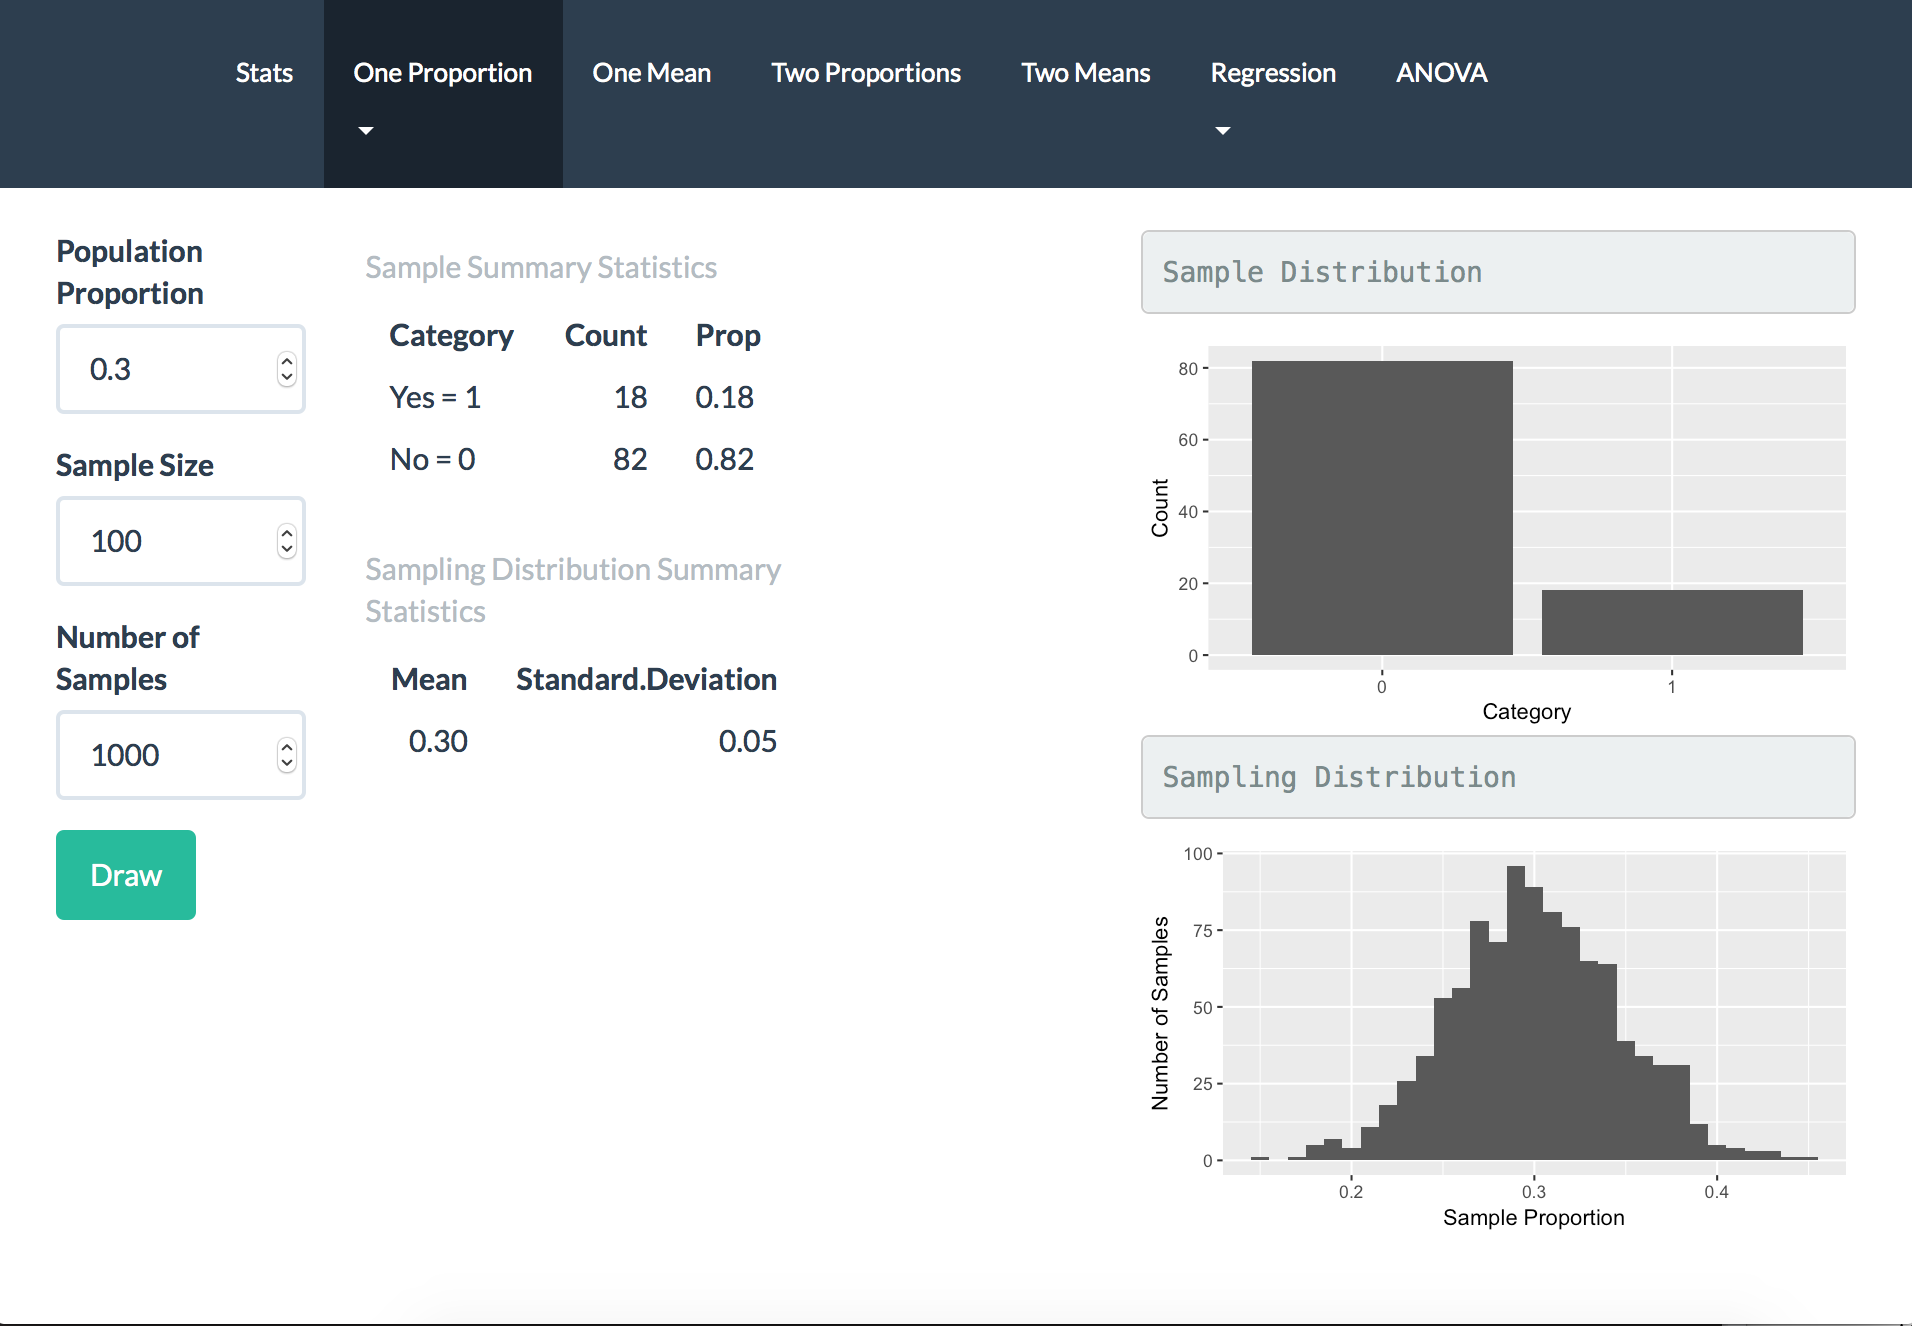
\includegraphics[width=\textwidth]{OneProp.png}
                \caption{Sampling Distribution Screen }
                \label{fig:OneProp}
        \end{subfigure}%

        \begin{subfigure}[b]{0.75\textwidth}
                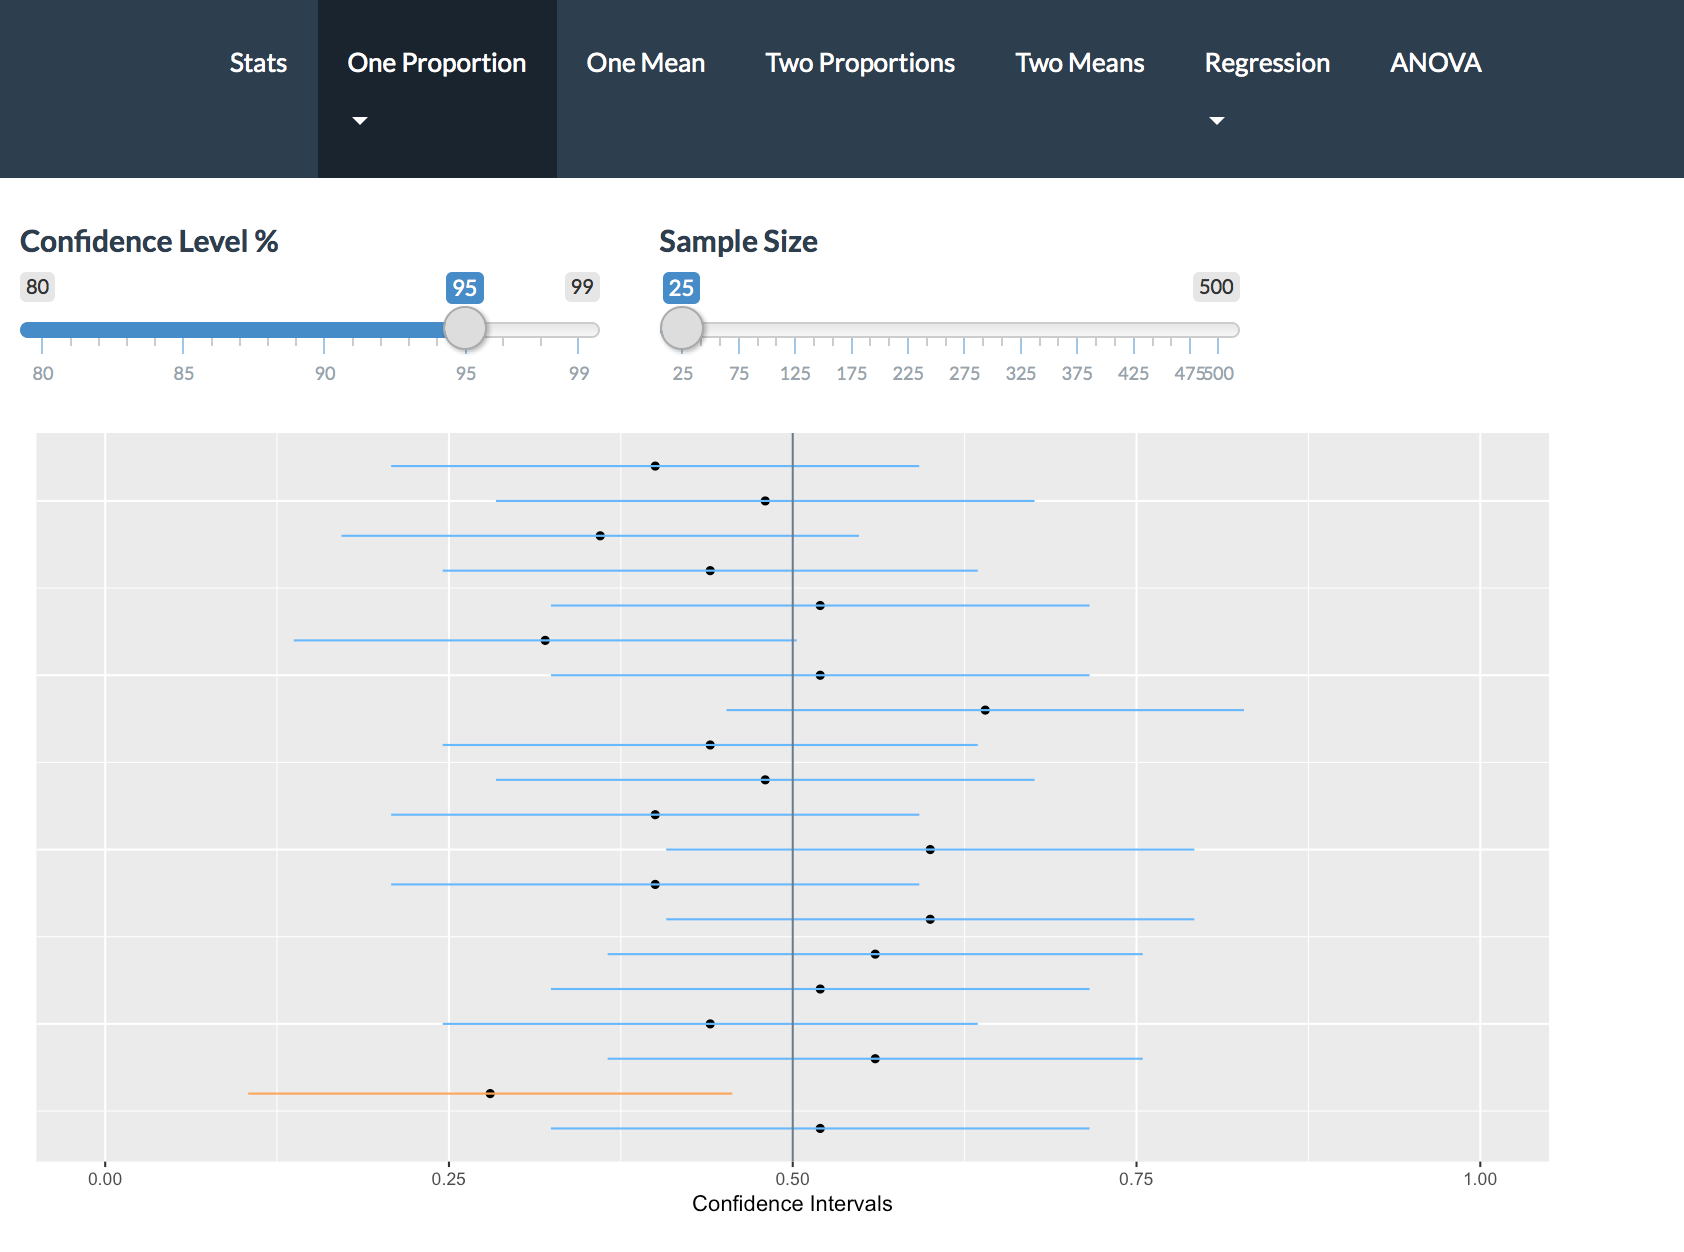
\includegraphics[width=\textwidth]{OnePropCI.png}
                \caption{Confidence Interval Screen} 
                \label{fig:OnePropCI}
        \end{subfigure}

\caption {Subsection of Inference for One Proportion.}
\end{figure}


\subsection{One Mean}
The section One Mean focuses on the concept of sampling distribution for one mean. They layout is similar to that of the inference for one proportion.  The inputs allow the user to enter the mean, standard deviation, sample size, and number of samples.  Once the "Draw" button is clicked, the sampling distribution begins to appear with summary statistics in addition to the last drawn sample distribution and its summary statistics. The samples are drawn from a normal distribution with the mean and standard deviation input by the user.   We can see a screen shot of this section in Figure~\ref{OneMean}.


\begin{figure}[H]
\centering
        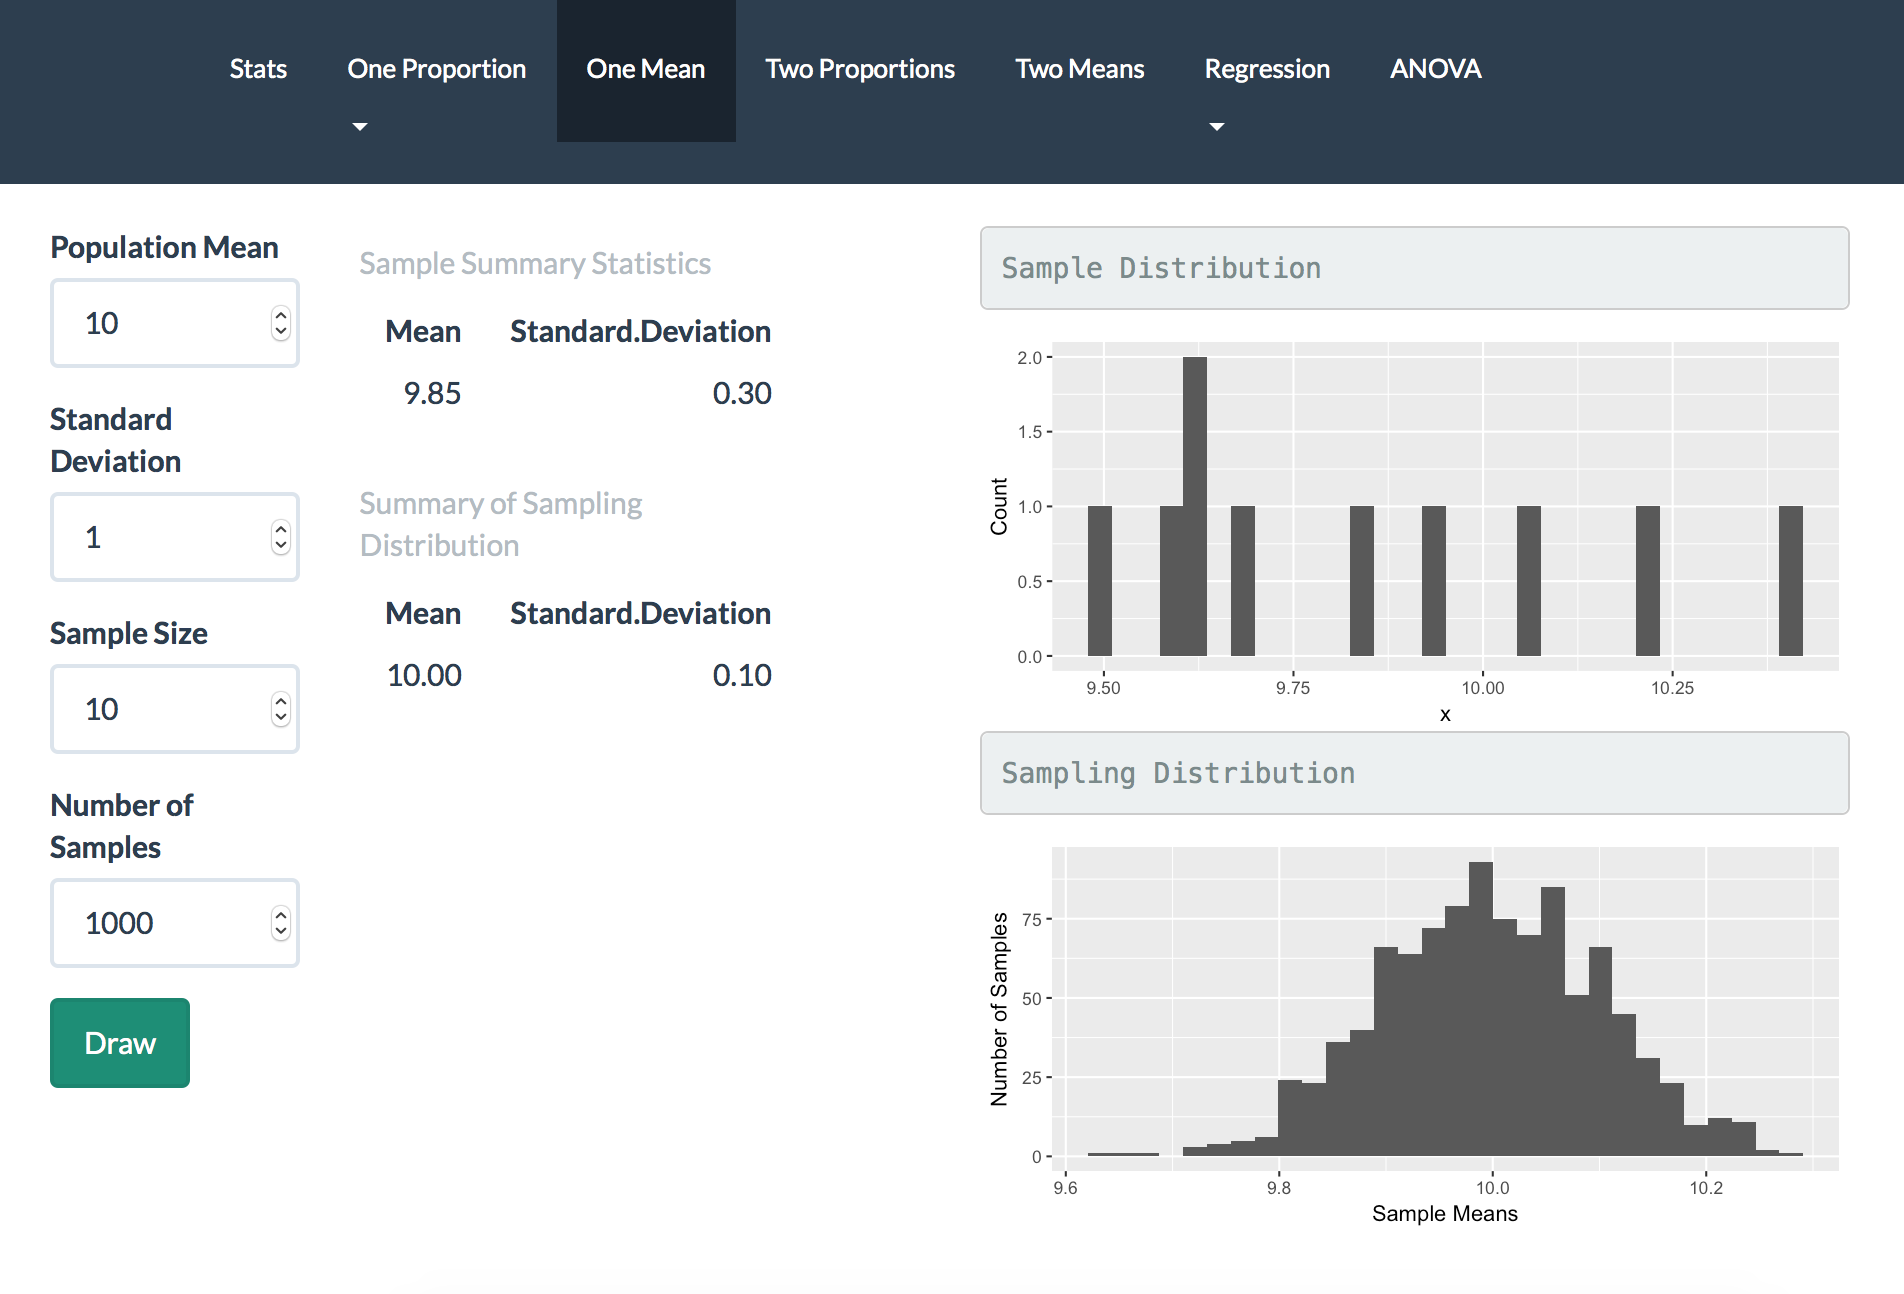
\includegraphics[width=\textwidth]{OneMean.png}
        \label{fig: OneMean}
\end{figure}

\subsection{Two Proportions and Two Means}

The sections for two proportions and two means are constructed similarly to the single proportion and single means sections, as seen in Figure~\ref{TwoProp}.  They each aim to display a sampling distribution of sample statistic differences. The two proportions tab allows the user to input the population proportion for two different groups, the sample size for those groups, and the number of samples they wish to draw. It then draws from a binomial with the specified parameters for each group. The results of the sample are shown in the Sample Distribution graphs. The table of Sample Summary information displays the proportion for each group as well as the difference in those proportions. The Sample Distribution graph is created by repeating this process many times and saving the differences in the two proportions each time. The summary information for the Sampling Distribution is displayed in the Sampling Distribution Summary table.

The Two Means tab recreates the same process except with calculating the difference in means for two different groups. The user can input a specific mean and standard deviation for each of the two groups. The samples will then be generated form a normal distribution with those specifications. The setup of this section is similar to that of Two Proportions where we are given both the Sample Distribution and the Sampling Distribution, in addition to tables that provide the summary statistics for those graphs.

\begin{figure}[H]
\centering
        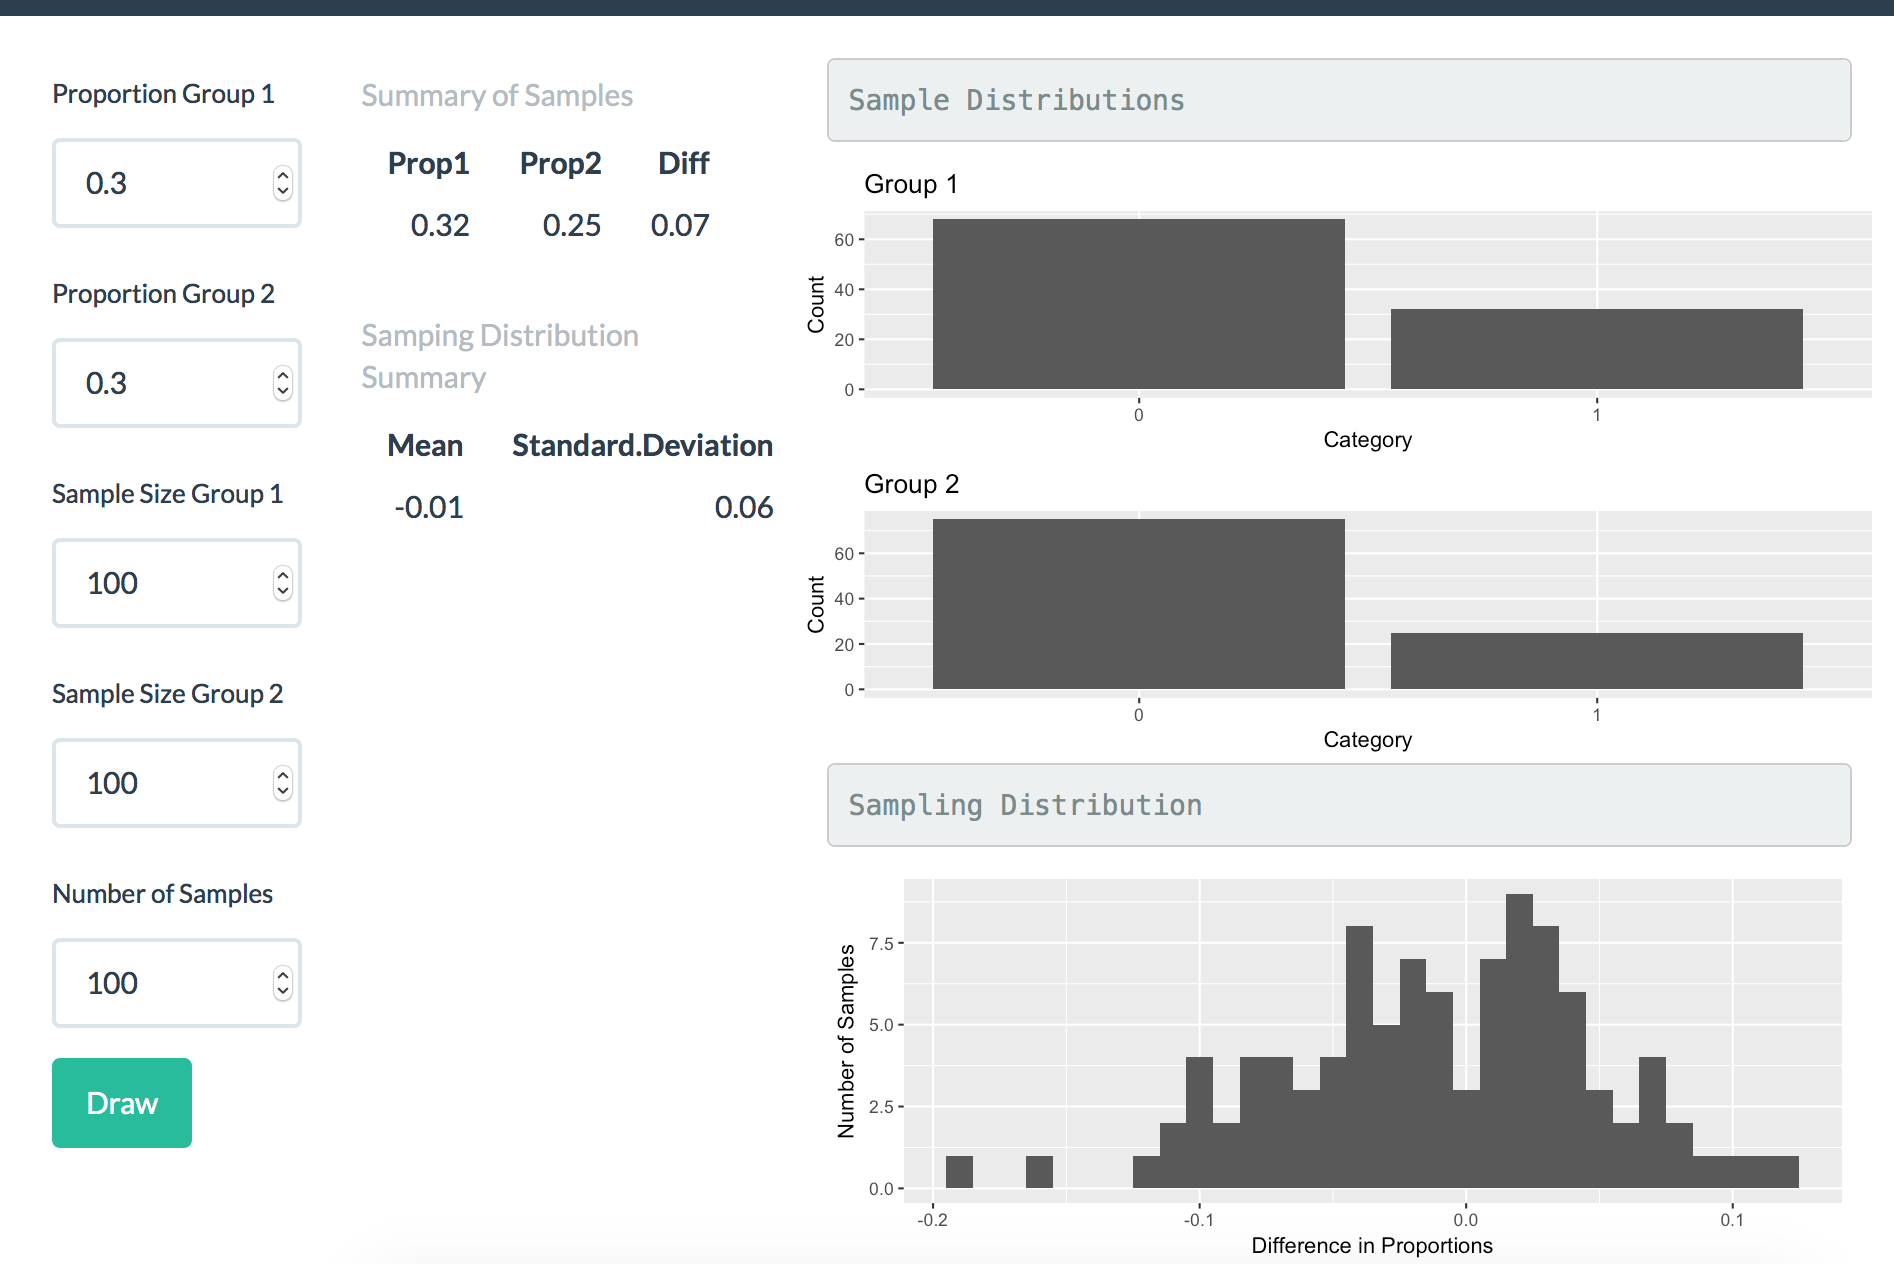
\includegraphics[width=\textwidth]{TwoProp.png}
        \label{fig:TwoProp}
\end{figure}


\subsection{Linear Regression: Correlation}
Another section featured in the Shiny application is based on linear regression topics. The correlation page features a slider that allows the user to select correlation values for a random plot of points. Figure~\ref{Correlation}  gives a a screen shot of this section of the Shiny app. This allows the user to see what different correlations look like ranging from -1 to 1. In order to make this plot, a multivariate normal random data frame is created that has 100 sets of data points designed with a specific sigma matrix.  This sigma matrix changes based on the user input correlation value, but keeps 1 as the variance for both x and y.  Thus, the XY coordinates are generated with a set correlation. These points are then plotted on the graph and update as the slider is moved. 

\begin{figure}[H]
\centering
        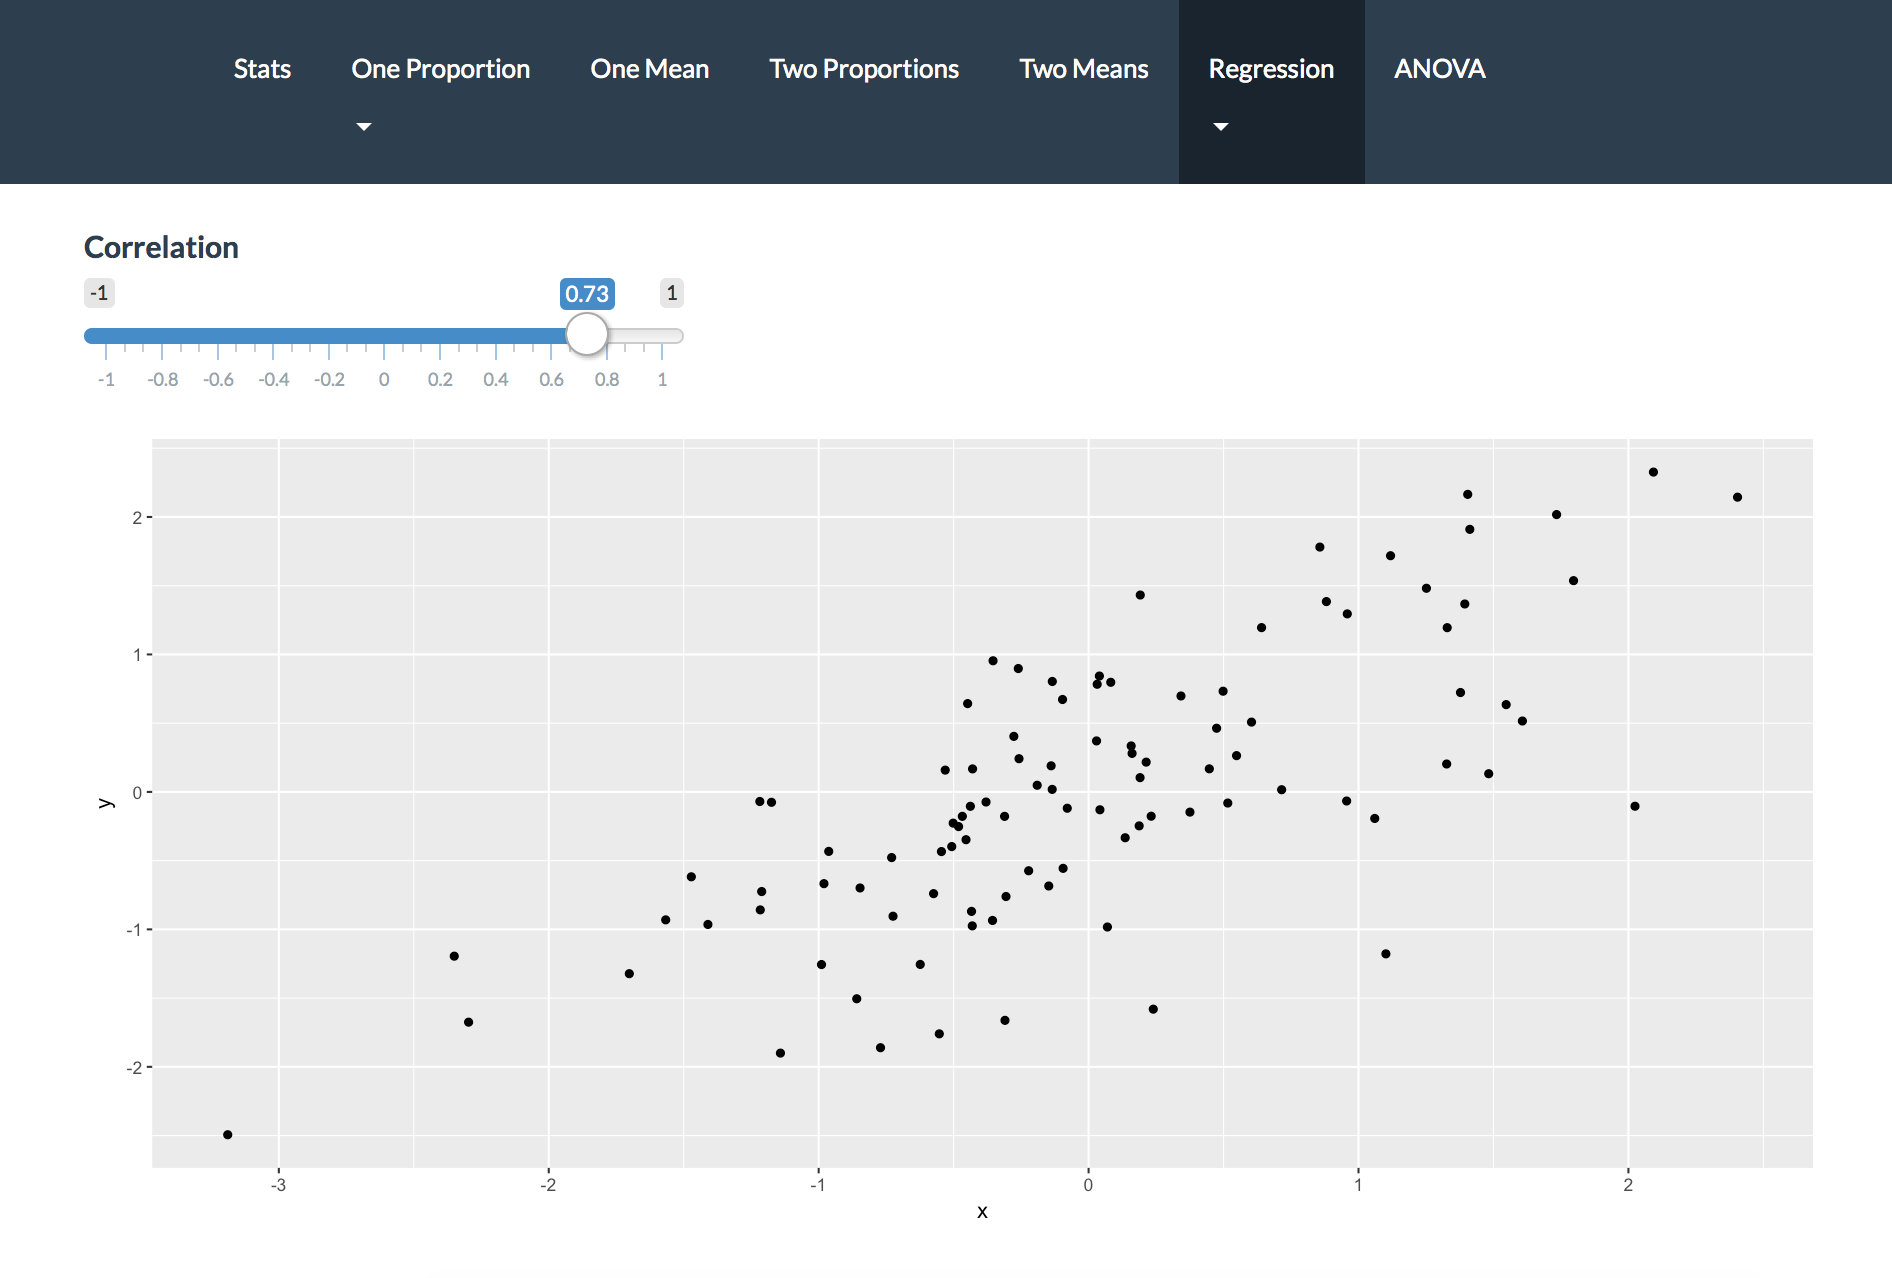
\includegraphics[width=\textwidth]{Correlation.png}
        \label{fig:Correlation}
\end{figure}



\subsection{Linear Regression: Outliers}
 
 The outliers tab under Linear regression is designed to display multiple data sets with varying outliers.  The data sets are all identical except for the one outlier point, which will be set in a red color.  Once a data set is selected the user can select to fit a line of least squares to the data, both with and without the outlier.  Once the box is checked to fit a line to the data, the line is placed on the graph, blue for the line fit with the outlier and green slashes for a line fit to the data without the outlier. The output will also display the intercept, slope and coefficient of determination for the lines on the graph.  
 
 \begin{figure}[H]
\centering
        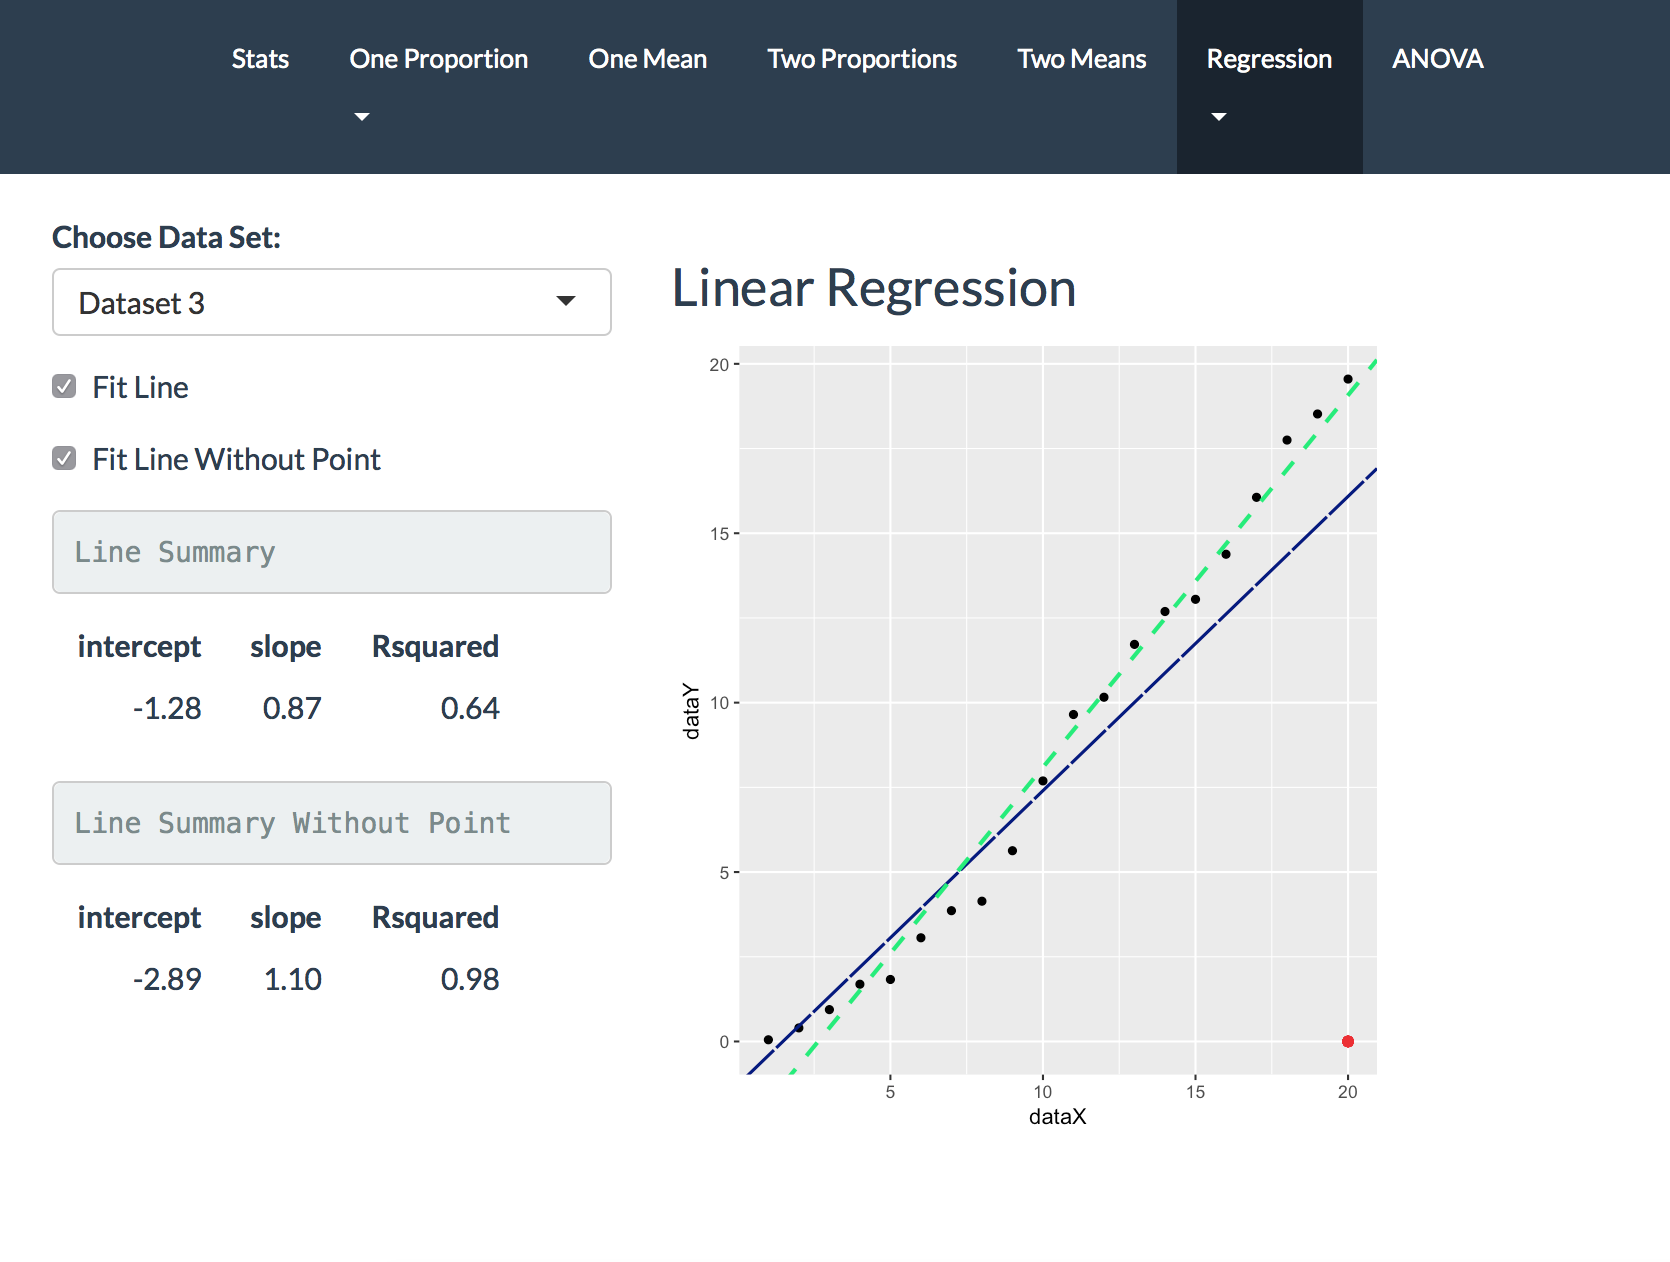
\includegraphics[width=\textwidth]{Outliers.png}
        \label{fig:Outliers}
        \caption{Outliers in Linear Regression}
\end{figure}

\subsection{Linear Regression: Equation}

The Equation section of the Shiny app breaks down the components of an equation and provides interpretations for intercepts and slopes.  In addition, the user can manipulate the intercept and slope of the points on the graph in order to see how it changes the points and the the line fit to them.  The data for this plot is generated using the same multivariate random normal data generating function in R as in the correlation section. This time, the input slope value is set as the correlation in the sigma matrix. The data is then adjusted to meet the intercept requirements by shifting the points created with the specific slope to pass through the user input intercept value. The data on the plot will update as the intercept and slope sliders are moved.  When the  ``Fit Line'' box is selected the equation for that least squares line will be displayed. It will have the same intercept and slope as the sliders display. The user can then select the "Intercept" box to see a red dot appear at the y-intercept on the plot. They will also be shown an intercept interpretation that is specific the the intercept they see in the plot. Similarly, when the "Slope" box is checked there is an interpretation of the slope that is output for the user.  The graph will display the rise and run of the slope to help illustrate the interpretation for the slope. A horizontal green line represents the one unit increase in the explanatory variable, while a vertical blue line indicates the increase or decrease in the response variable as a result of the increase in the explanatory variable. The user can manipulate the sliders and the check boxes as they see fit, and the plot and output will continually update. Figure~\ref{LinEq} displays the screen for Equation when all boxes are checked. 

\begin{figure}[H]
\centering
      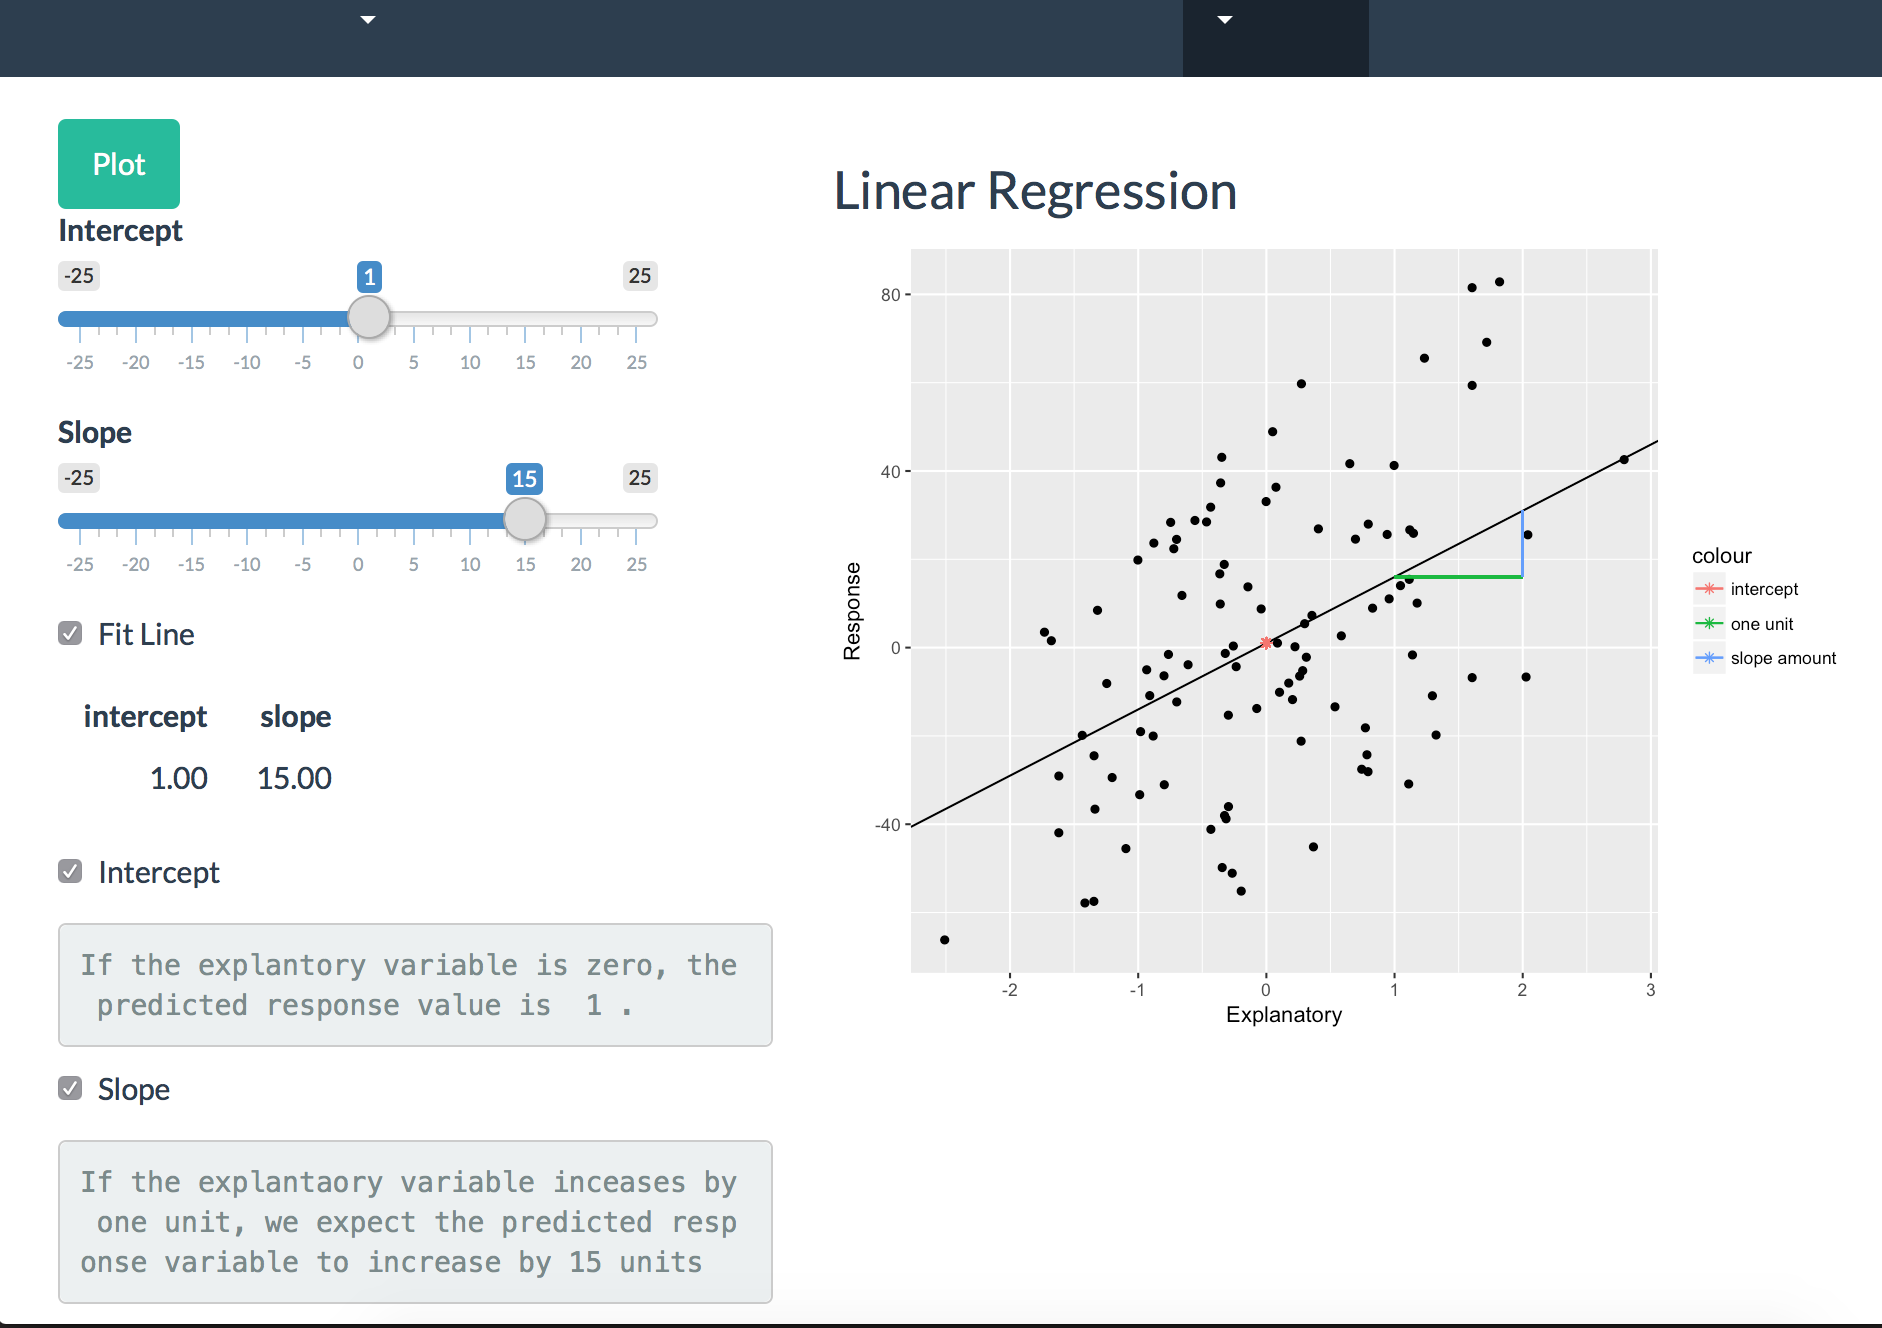
\includegraphics[width=\textwidth]{LinEq.png}
      \label{fig: LinEq}
      \caption{Equation Tab}
\end{figure}

\subsection{ANOVA}

The last tab of the shiny application is the ANOVA tab.  This tab explores the relationship among the means of 3 different groups.  The user can input the means, standard deviations, and sample sizes for each of the three groups. This can be seen in Figure~\ref{ANOVAUP}. Then R will generate the samples for each group using a normal distribution with the input parameters for each group. Then, the graph will display a dotplot for each of those groups.  Next to the graph, is an ANOVA table for the differences in the means along with the summary information for each of the three groups. The output for this part of the Shiny app can be seen in Figure~\ref{ANOVALOW}.

\begin{figure}[H]
        \centering

        \begin{subfigure}[b]{0.75\textwidth}
                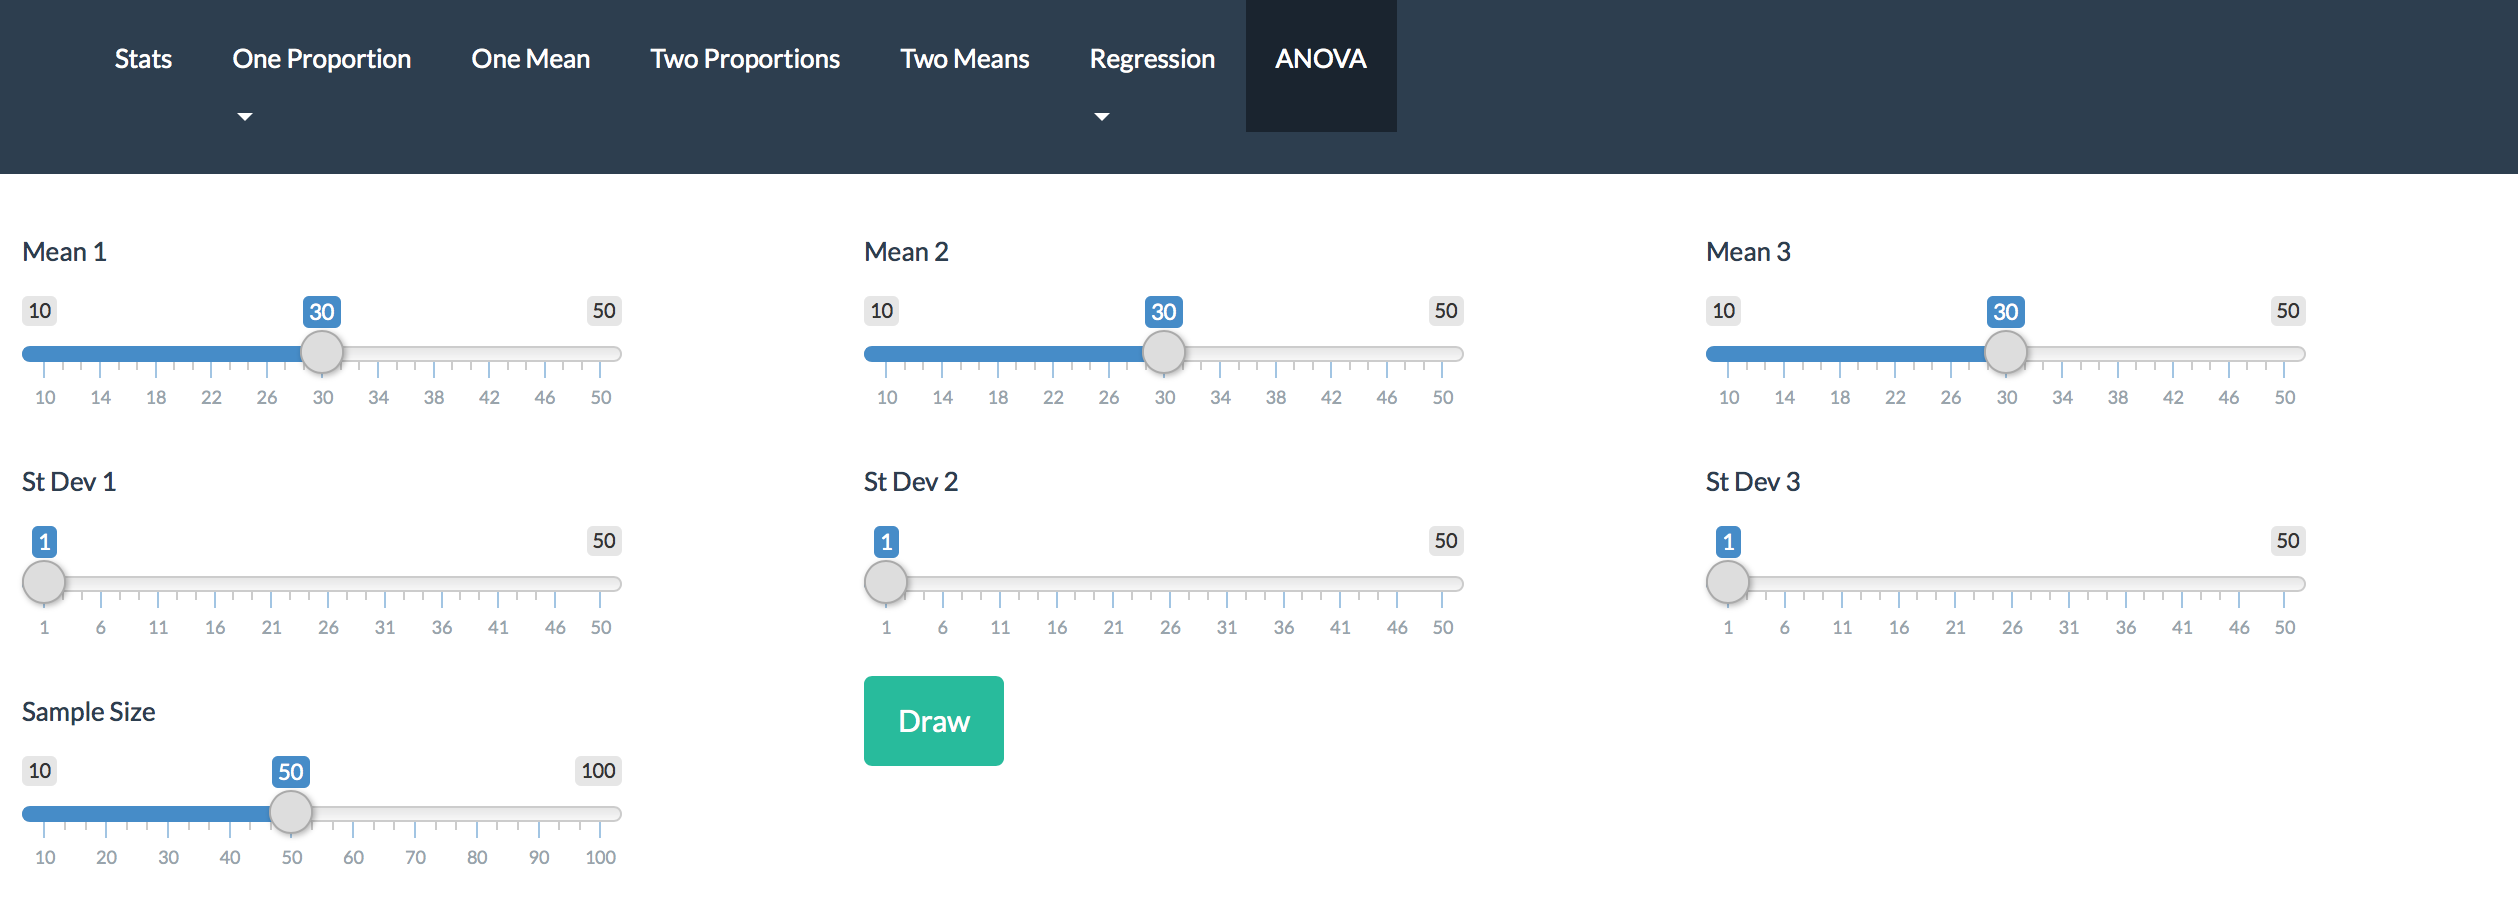
\includegraphics[width=\textwidth]{ANOVAUP.png}
                \caption{ANOVA Section top }
                \label{fig:ANOVALOW}
        \end{subfigure}%

        \begin{subfigure}[b]{0.75\textwidth}
                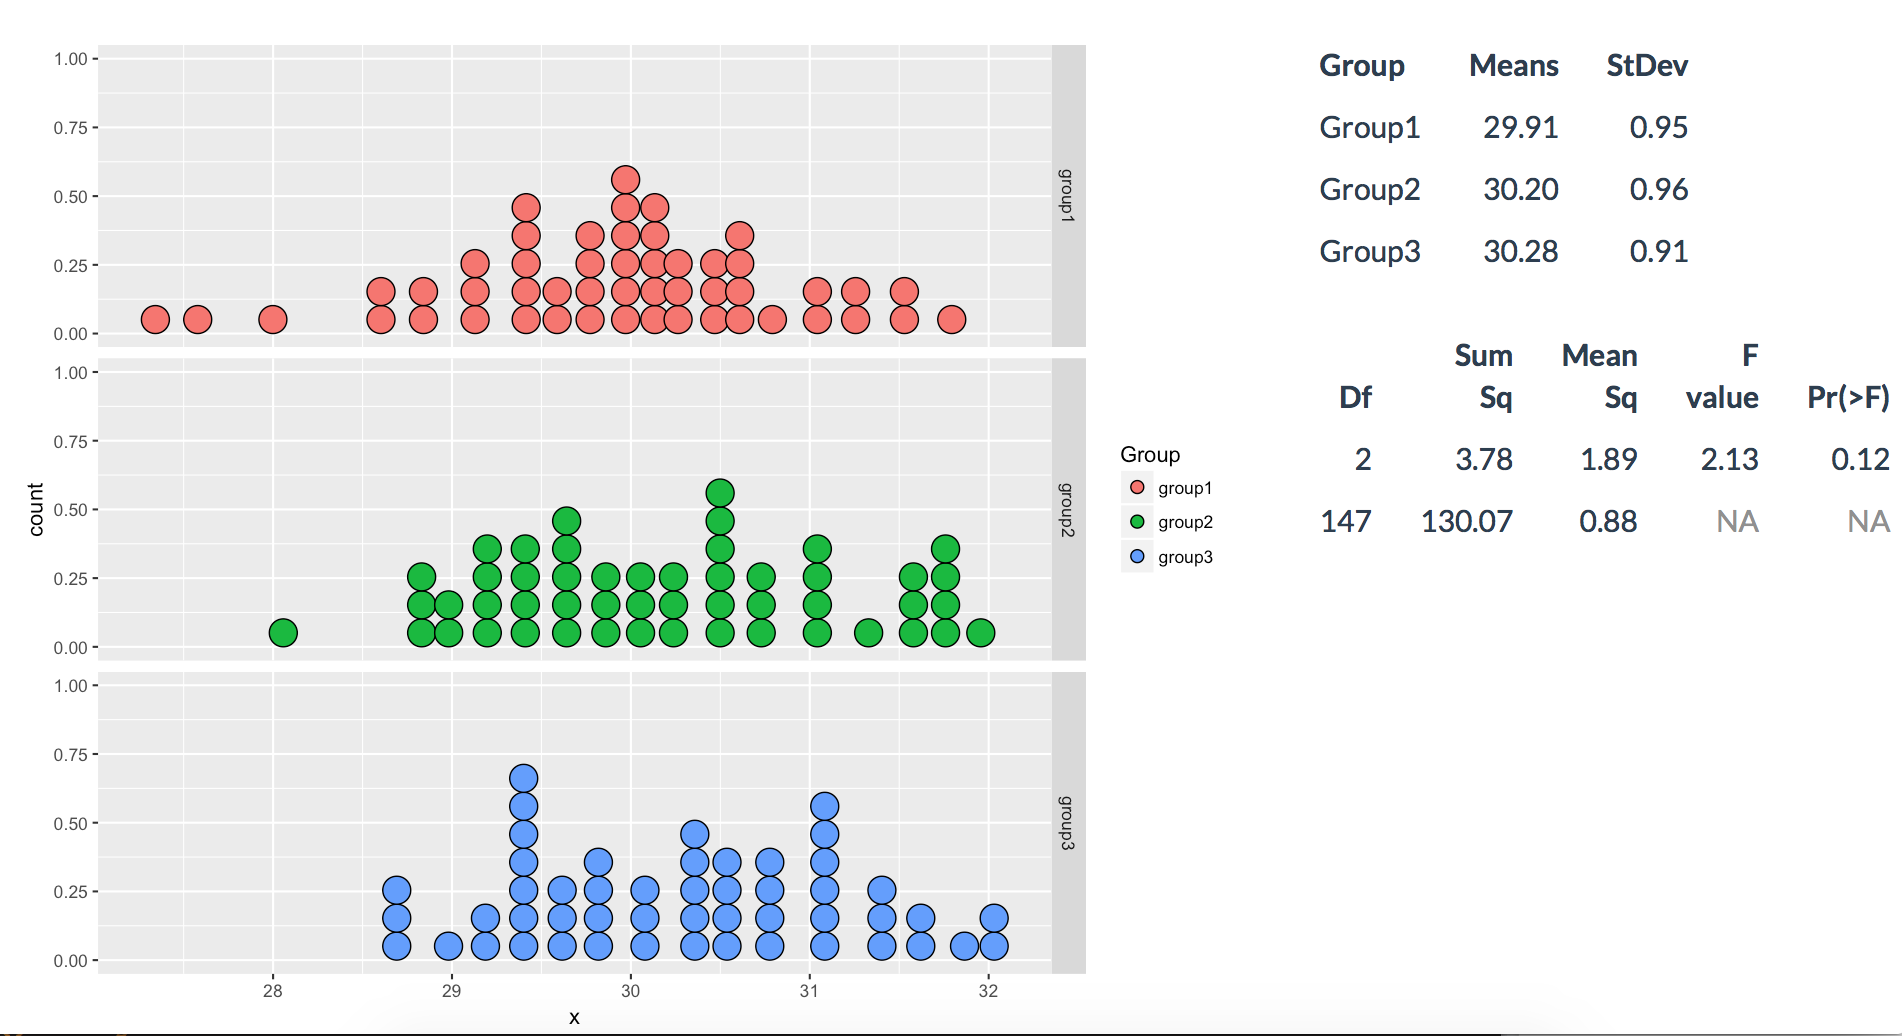
\includegraphics[width=\textwidth]{ANOVALOW.png}
                \caption{ANOVA Section lower} 
                \label{fig:ANOVALOW}
        \end{subfigure}

\caption {ANOVA Sections}
\end{figure}


\section{Conclusions and Future Work}
% These are the things that I have that other things don't
%based in R its free, independtent and runs on the web so everyone can use it, it has interactive features (could bullet point this)  
% Then talk about where it goes next
%different options in the tabs could be built into the app for hyp test or other similar topics 
%Software testing over the next few month from students in intro stats and high school and community college math teachers on the software
\section{References}


 \begin{thebibliography}{1}

\bibitem{chance}  Chance, B., Ben-Zvi, D.,$\&$ Garfield, J.,  Medina, E. (2007). The Role of Technology in Improving Student Learning of Statistics.

\bibitem{doi}  Doi, J., Potter G., Wong J., Alcaraz I., $\&$ Chi, P. (2016). Web Application Teaching Tools for Statistics Using R and Shiny. 

\bibitem{Pea} Roy D. Pea. Cognitive Technologies for Mathematics Education. A. Schoenfeld. Cognitive science and mathematics education. Hillsdale, pp.89-122, 1987. $<$hal-001990547$>$

\bibitem{Rossman} Rossman, A.$\&$ Chance, B. (2004), The \emph{Rossman/Chance Applet Collection}. Available at www.rossmanchance.com/applets.


  \end{thebibliography}



\subsection{Worksheets}

Another component of this project was creating worksheets that correspond to each of the sections of the Shiny app. Though the app can stand alone to help vizualize various topics, the worksheets walk the user through using each section and try to help illustrate ideas. The worksheets for each section work to help demonstrate the following ideas:
\begin{itemize}

\item One Proportion and One Mean: Leads user through drawing one sample and seeing how it is displayed in the Sample Distribution vs in the Sampling Distribution. Then, leads to drawing more samples and seeing that the Sampling Distribution ends up centered around population proportion.  

\item   Confidence Interval: Walk the user through fixing the confidence level and seeing what happens to the width of the intervals as the sample size in increased from 25 to 500. In the second question the sample size is fixed at 250 and the confidence level is increased from 80 to 99$\%$.  Through manipulation of these two components the user is quickly able to see the relationship between confidence interval width, the sample size, and the confidence level.
  
\item   Two Proportions and Two Means: takes the user the student through taking multiple samples to build the sampling distribution which ends up being approximately normal, similar to the one proportion and one mean inference sections.
  
\item   Corrleation: takes the user through observing the structures of the data as the slider moves from a correlation of -1 to 1. They will take note of the direction and form of the data as the correlation changes. 

\item Outliers: leads the user through the linear model selection process of fitting data both with and without an outlier and determining which model best fits the data.  Users will also look at multiple outliers and determine whether they have high leverage, high residual or both.

\item Equation: guides the user through manipulating the slope and intercept on the plot and porviding interpretations of those values.
  
\item   ANOVA:  gives the user a small introduction to the ANOVA F test followed by some questions asking them to explore the relationship between the mean, standard deviation, sample size and the resulting p-value and conclusion to the F-test. 
\end{itemize}
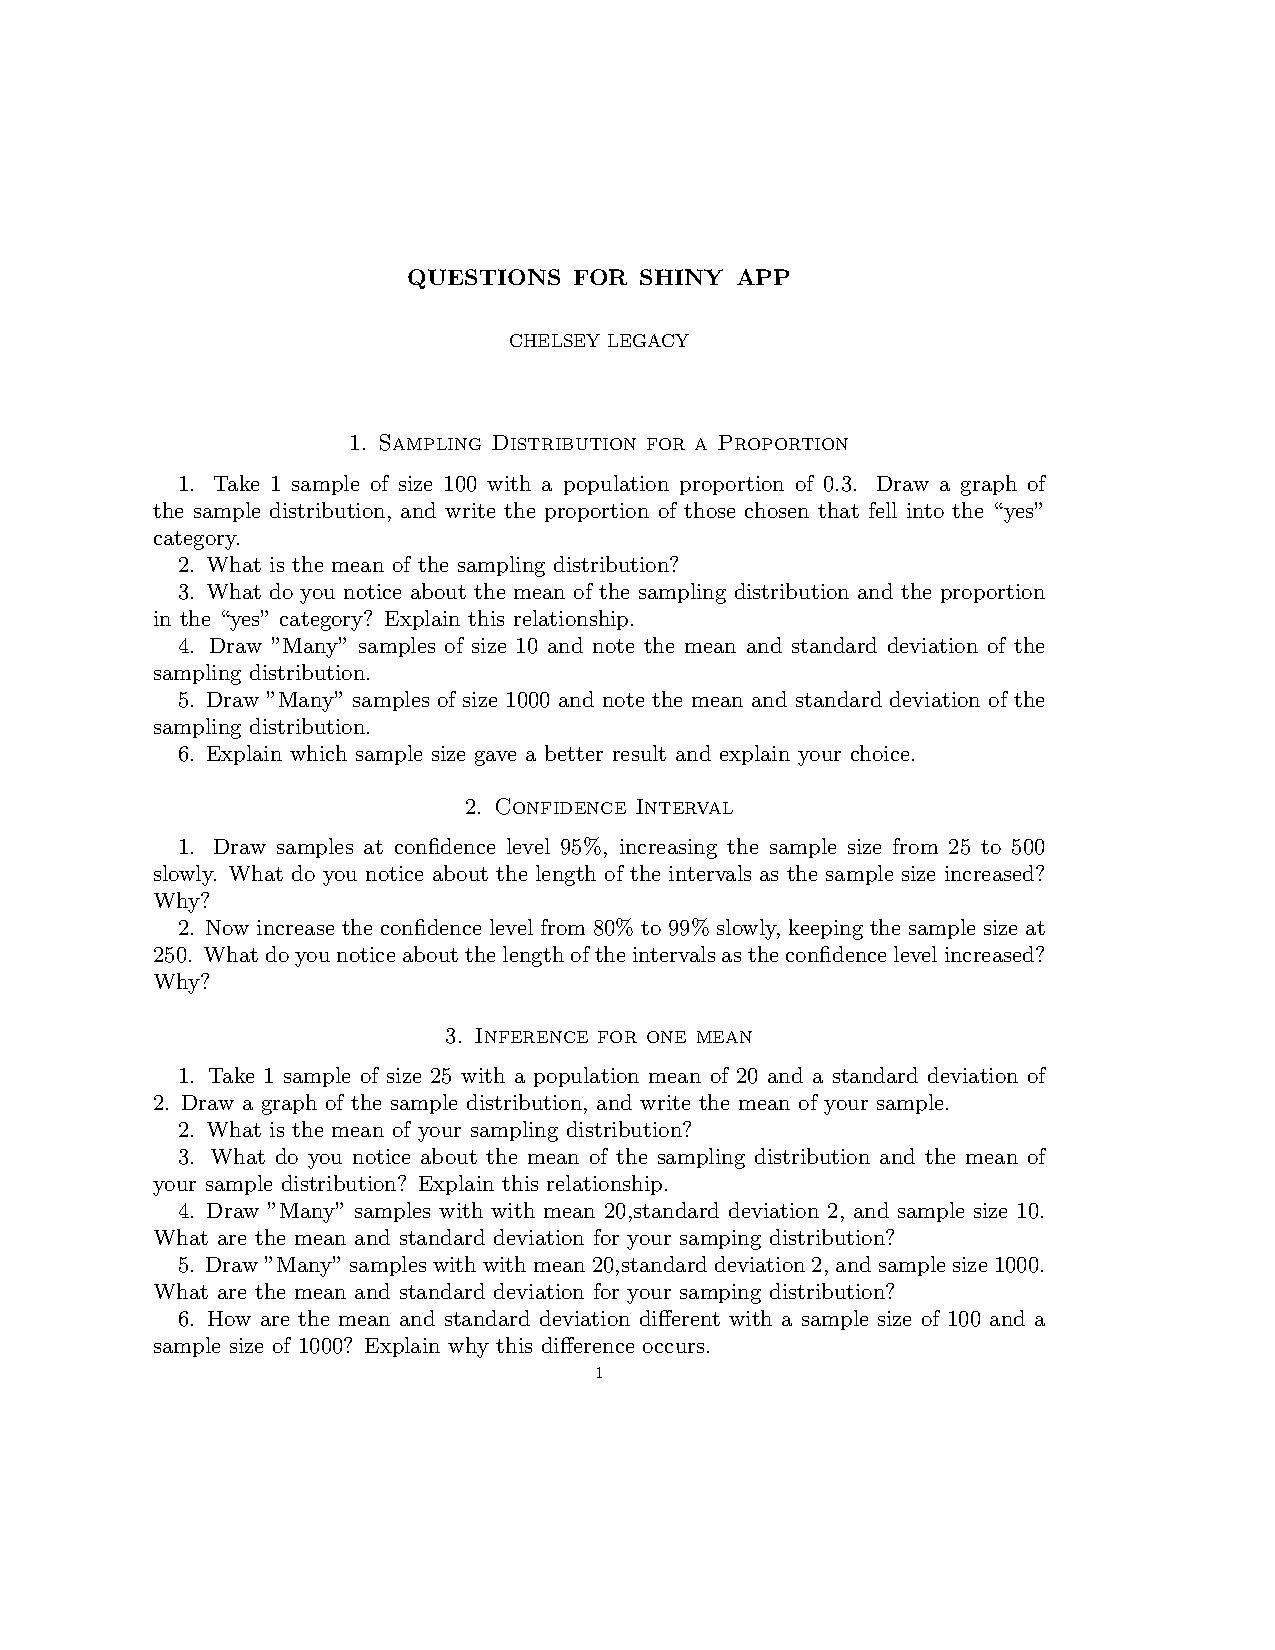
\includepdf[pages=-]{Questions.pdf}








\end{document}
\end

